% Two slides: network parameters over 2016-2026 compared with the random-tree baseline.
% To use in the main deck: copy the two frames below, the figures/ folder,
% and the packages marked "needed by the frames" into the main preamble.
\documentclass[aspectratio=169]{beamer}

% needed by the frames
\usepackage{amsmath}
\usepackage{booktabs}
\graphicspath{{figures/}}

\setbeamertemplate{navigation symbols}{}

\begin{document}

% ---------------------------------------------------------------- slide 1
\begin{frame}{Real network vs random trees, 2016--2026}
\begin{columns}[c,onlytextwidth]
\begin{column}{0.76\textwidth}
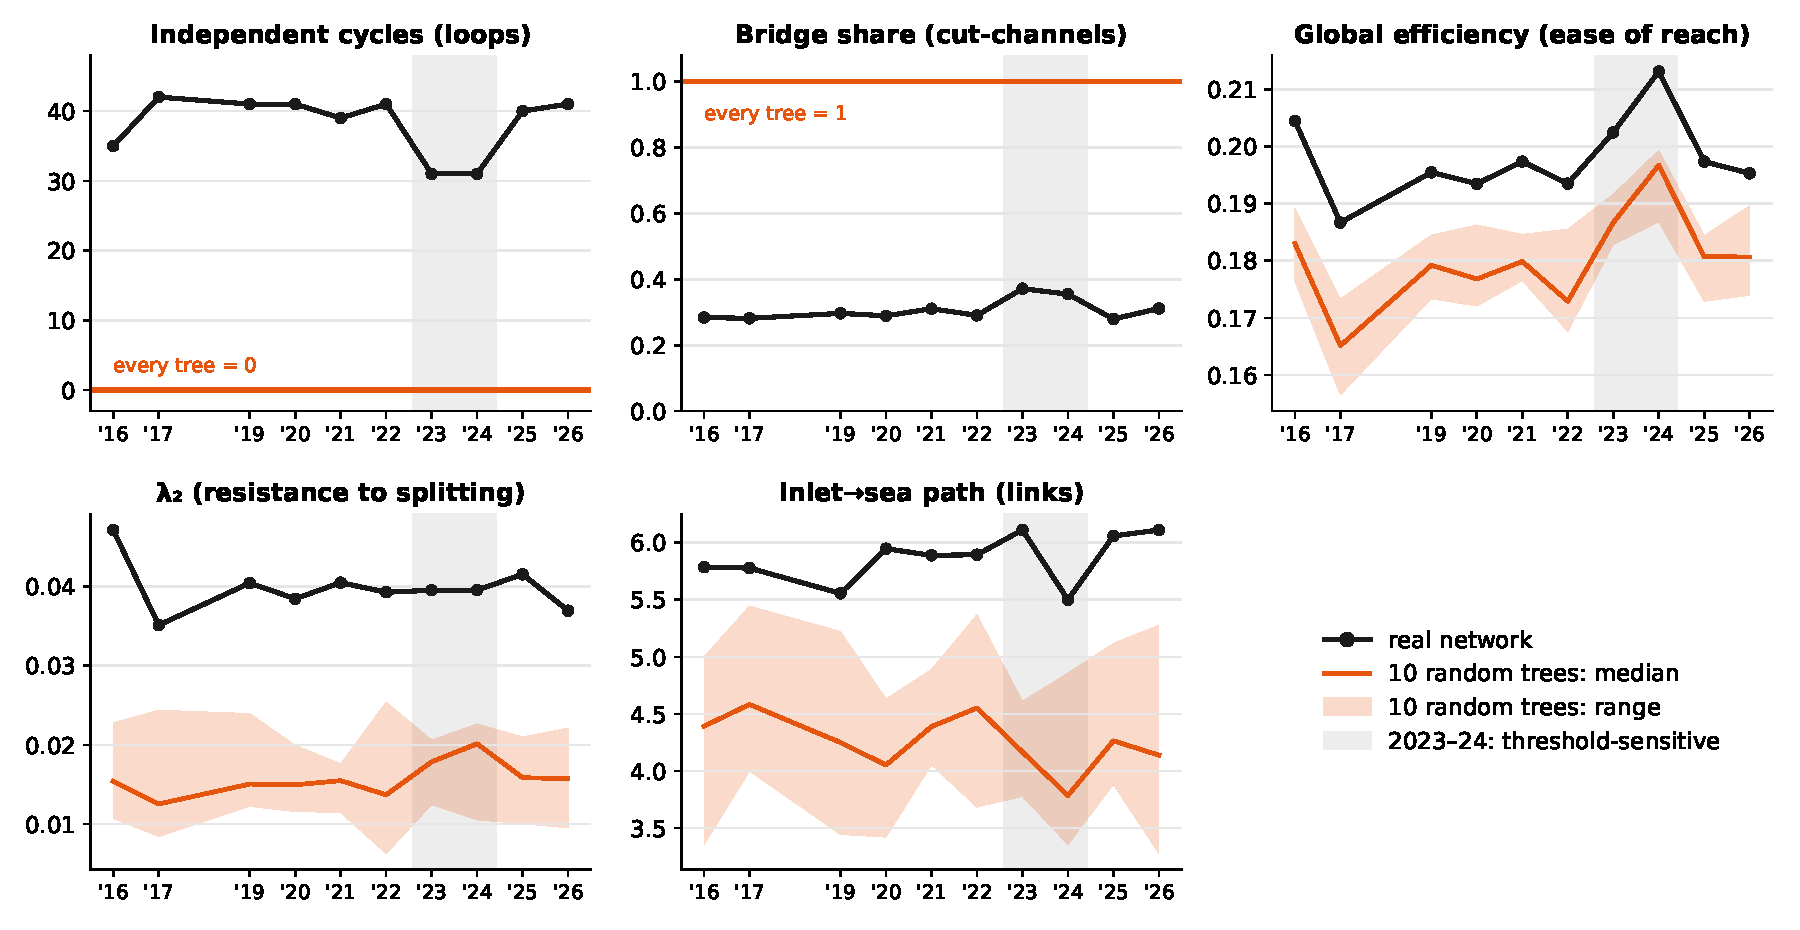
\includegraphics[width=\linewidth]{comparison_5.pdf}
\end{column}
\begin{column}{0.23\textwidth}
\footnotesize
\begin{itemize}\setlength{\itemsep}{6pt}
  \item \textbf{Loops:} 31--42 a year; trees 0.
  \item \textbf{Bridges:} 28--37\%; trees 100\%.
  \item \textbf{Efficiency, $\lambda_2$, path:} beyond all 10 trees, every year.
\end{itemize}

\vspace{3mm}
\alert{Far more connected and redundant than a tree.}
\end{column}
\end{columns}
\end{frame}

% ---------------------------------------------------------------- slide 2
\begin{frame}{Trends over ten years}
\begin{columns}[c,onlytextwidth]
\begin{column}{0.60\textwidth}
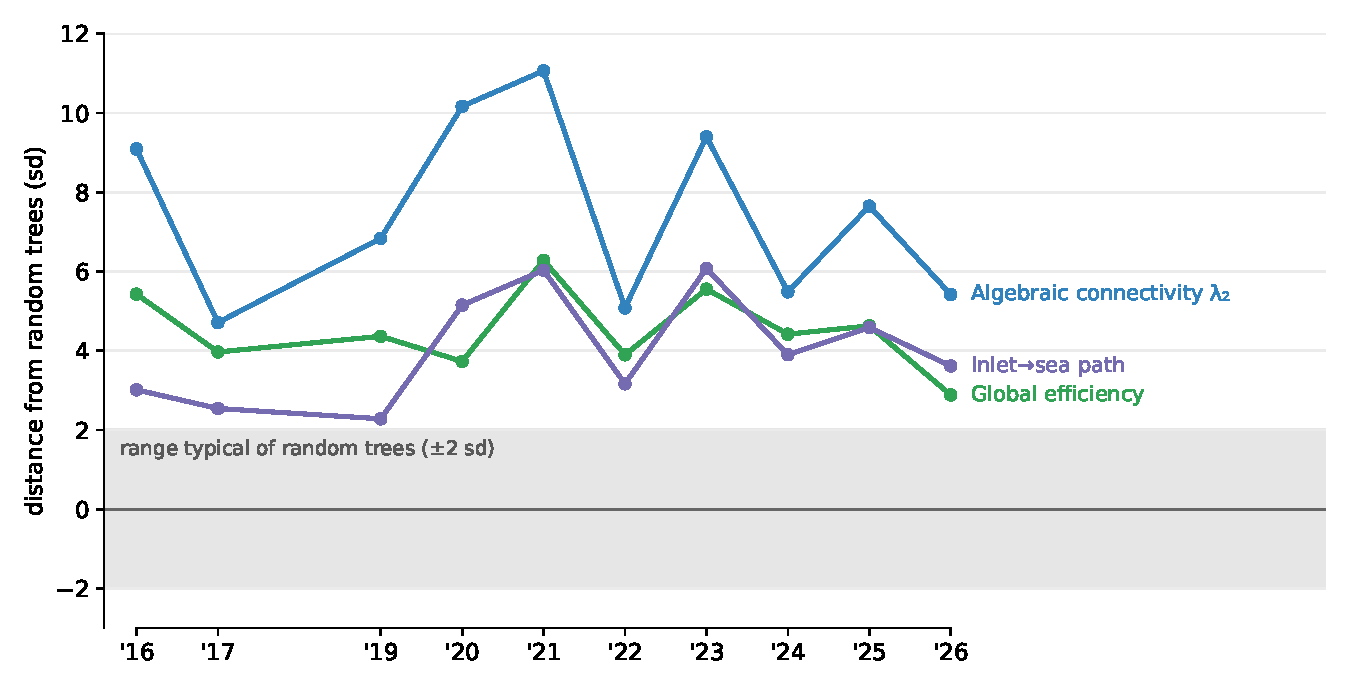
\includegraphics[width=\linewidth]{zscores.pdf}
\end{column}
\begin{column}{0.38\textwidth}
\small
\begin{tabular}{@{}lrr@{}}
\toprule
Parameter & Kendall $\tau$ & $p$ \\
\midrule
Independent cycles & $-0.19$ & 0.46 \\
Bridge share & $+0.33$ & 0.22 \\
Global efficiency & $+0.16$ & 0.60 \\
$\lambda_2$ & $-0.02$ & 1.00 \\
Inlet$\to$sea path & $+0.40$ & 0.11 \\
\bottomrule
\end{tabular}

\vspace{3mm}
\begin{itemize}\setlength{\itemsep}{4pt}
  \item No significant trend in any parameter.
  \item The gap to the trees stays large: $+2$ to $+11$ sd.
  \item The 2023--24 dip in loops depends on the water threshold.
\end{itemize}
\end{column}
\end{columns}
\end{frame}

\end{document}
